\documentclass[12pt,twoside]{report}
\usepackage[utf8]{inputenc}
\usepackage{titlesec, amsmath, amsfonts, pgf, tikz, adjustbox, filecontents, 
graphicx, wrapfig, relsize, float, mathtools, appendix, array, algorithm2e, 
siunitx, bbm}
\usepackage{pgfplots}
\usepackage[font=small, labelfont=it]{caption}
\usepackage[font=small, labelfont=normalfont, 
justification=centering]{subcaption}
\usepackage[margin=1.5in]{geometry}
\renewcommand{\baselinestretch}{1.5}
\usetikzlibrary{arrows, automata, positioning, quotes, arrows.meta, spy, 
shapes.geometric}

\tikzset{
  annotated cuboid/.pic={
    \tikzset{%
      every edge quotes/.append style={midway, auto},
      /cuboid/.cd,
      #1
    }
	\draw [every edge/.append style={pic actions, densely dashed, opacity=.5}, 
	pic actions]
    (0,0,0) coordinate (o) -- ++(-\cubescale*\cubex,0,0) coordinate (a) -- ++(0,-\cubescale*\cubey,0) coordinate (b) edge coordinate [pos=1] (g) ++(0,0,-\cubescale*\cubez)  -- ++(\cubescale*\cubex,0,0) coordinate (c) -- cycle
    (o) -- ++(0,0,-\cubescale*\cubez) coordinate (d) -- ++(0,-\cubescale*\cubey,0) coordinate (e) edge (g) -- (c) -- cycle
    (o) -- (a) -- ++(0,0,-\cubescale*\cubez) coordinate (f) edge (g) -- (d) -- cycle;
    \path [every edge/.append style={pic actions, |-|}]
    (b) +(0,-5pt) coordinate (b1) edge ["\xunits"'] (b1 -| c)
    (b) +(-5pt,0) coordinate (b2) edge ["\yunits"] (b2 |- a)
    (c) +(3.5pt,-3.5pt) coordinate (c2) edge ["\zunits"'] ([xshift=3.5pt,yshift=-3.5pt]e)
    ;
  },
  /cuboid/.search also={/tikz},
  /cuboid/.cd,
  width/.store in=\cubex,
  height/.store in=\cubey,
  depth/.store in=\cubez,
  xlabel/.store in=\xunits,
  ylabel/.store in=\yunits,
  zlabel/.store in=\zunits,
  scale/.store in=\cubescale,
  width=10,
  height=10,
  depth=10,
  scale=.1,
}

\tikzset{
    annotated square/.pic={
        \tikzset{%
            every edge quotes/.append style={midway, auto},
            /square/.cd,
            #1
        }
        \draw (0,0,0) -- node[above]{\xlabel} ++ (-\x*\scale,0,0) -- node[left]{\ylabel} ++ (0, -\y*\scale, 0) -- ++ (\x*\scale,0,0) -- cycle;
    },
    /square/.search also={/tikz},
    width/.store in=\x,
    height/.store in=\y,
    scale/.store in=\scale,
    xlabel/.store in=\xlabel,
    ylabel/.store in=\ylabel,
    scale=.1,
}



\def\arraystretch{.8}

\newcolumntype{T}[1]{S[table-format=#1]}

\newcommand{\ubb}[4][]{\underset{#3 \times #4}{\mathbb{#2}_{#1}}}

\newcommand{\mc}[1]{\multicolumn{1}{c|}{#1}}
\newcommand{\figref}[1]{Figure \ref{#1}}
\newcommand{\Figref}[1]{Figure \ref{#1}}

\newcommand{\adjacencyT}[3]{%
	\begin{tabular}{cccc}
		& 0 & 1 & 2\\\cline{2-4}
		\mc{0} & #1\\
		\mc{1} & #2\\
		\mc{2} & #3
	\end{tabular}
	}

\renewcommand\theequation{\bfseries\thechapter.\arabic{equation}}

\titleformat{\chapter}[hang]
{\normalfont\huge\bfseries}{\ \thechapter}{1em}{}
% for some reason this leaves the chapter number slightly bumped to the right

\title{
	{\huge{Neural Network Reconstruction via Graph Locality-Driven Machine 
	Learning}}\\
    {\large Bard College}
}
\author{Hayden Sartoris}
%\date{April 2018}
\date{}

\begin{document}

\maketitle
\tableofcontents
\listoffigures

\begin{abstract}
A ubiquitous problem within the field of computational neuroscience is the 
determination of biological neural network structure and connectivity from 
imaging of stochastic, large-scale network activity. We propose a machine 
learning algorithm inspired by convolutional approaches to image processing, 
adapted to the graph structure of neural networks. To achieve this, we redefine 
locality in terms of graph adjacency, and create a scale-independent algorithm 
facilitated by modern machine learning techniques to incorporate this locality 
data into individual connection prediction.
\end{abstract}


%! TEX root = /home/hsartoris/sproj/writeup/main.tex

\chapter{Introduction}

Artifical neural network-based solutions emerging in recent years have become a 
preeminent method for achieving accurate reconstructions of biological neural 
networks.\cite{Ray2015} However, the methods used tend to not take advantage of 
features unique to biological neural networks that can assist in producing 
reconstructions.  We present an architecture for determining network structure 
inspired by convolutional neural networks.  Whereas in image processing, the 
typical use case for convolutional networks, pixel and feature adjacency 
correlates with shared meaning, there exists no such metric for data extracted 
from biological neural networks, as per-neuron spike trains can be reconfigured 
into various permutations without necessitating a change in the structure of the 
network that generated those spikes. Thus our architecture redefines adjacency 
to a version more suited to the unique features of biological neural networks, 
derived from locality within the original graph structure.


%! TEX root = /home/hsartoris/sproj/writeup/main.tex
\graphicspath{{resources/}}

\chapter{Background}

\section{Biological Neural Networks}
\label{sec:bioNN}
Biological neural networks in the sense we will refer to them  here are 
collections of neurons, the connections between which enable cognition. Neurons 
themselves consist of a cell body, from which emerge axons and dendrites. Axons 
extend from the neuron body to meet the dendrites emerging from another neuron, 
and this forms an electrochemical one-way connection.\footnote{This is something 
	of an oversimplification, but it will suffice for our purposes; see 
	\cite{Reimann2017}} Neurons may connect to and receive connections from many 
	other neurons, and the axons can be so long as to render physical adjacency 
	of neurons in a network irrelevant in terms of connection 
	probability.\cite{axonlens}

\subsection{Neuron Behavior}
Neurons generally sit at a resting voltage, but upon receiving a high enough 
total input level from incoming connections to exceed a particular threshold, 
they spike, rapidly increasing in voltage and then dropping again. 
\cite{actionpotential} This voltage travels down the neuron's axons and in turn 
provides input to other neurons.
\subsection{Extracting Data}
Due to the three-dimensional nature of most brains, the sheer quantity of 
neurons, and their small size, manually mapping out a brain, and in particular 
the actual connections from neuron to neuron, is practically impossible. In 
order to monitor activity within a biological neural network, then, some 
compromises must be made. Several techniques exist for neuron monitoring; on the 
very small scale is the patch clamp technique, in which a pipette is directly 
attached to a single neuron\cite{neher1992patch}; on the larger scale is in-vivo 
calcium imaging, in which a dye is injected into a living brain, leading the 
neurons to fluoresce when spiking\cite{Stosiek7319}. As calcium imaging allows 
observation of as many neurons as can be seen by a camera, we are interested in 
data that are derived from this process.

\begin{wrapfigure}[8]{r}{.25\textwidth}
	\centering
	\vspace{-14pt}
	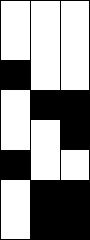
\includegraphics[width=.13\textwidth]{models/3neurEx/fullRun/1_dumb/input.png}
	\captionsetup{width=.85\linewidth}
	\caption{Spike time raster plot}
	\label{fig:rasterplot}
\end{wrapfigure}
Although calcium uptake into neurons during spiking is relatively slow, making 
determination of precise spike time difficult, use of existing deconvolution 
algorithms can facilitate the creation of spike-time raster plots\cite{Xu8025}.  
These plots contain a binary representation of neuron spiking: at each timestep, 
each neuron is either spiking, or not. In \figref{fig:rasterplot}, each column 
corresponds with one neuron, and each row represents a timestep; a filled block 
indicates a spike, and an unfilled block indicates no spike.


\section{Graphs}
In general, we define a graph as a collection of nodes and edges, where nodes 
represent states or components of a system, and edges represent the connections 
between those nodes\cite{networksciencebook}. An example graph can be found in 
\figref{fig:digraph}.

\begin{wrapfigure}[6]{l}{.28\textwidth}
	\centering
	\vspace{-5pt}
	
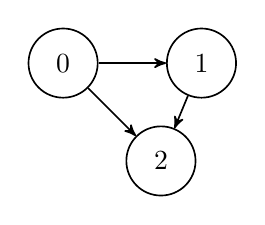
\begin{tikzpicture}[baseline=(current bounding box.center),->,>=stealth', 
	node distance=5em, semithick]
	\tikzstyle{every state}=[fill=none, draw=black, text=black]

	\node[state] (0) {0};
	\node[state] (1) [right of=0] {1};
	\node[state] (2) [below right of=0] {2};

	\path 	(0) edge node {} (1)
			(0) edge node {} (2)
			(1) edge node {} (2);
\end{tikzpicture}

	\caption{Digraph}
	\label{fig:digraph}
\end{wrapfigure}
\noindent Graphs can be used to describe many systems; for example, social 
groups can be represented in graph form, where people are nodes and friendships 
are edges.  In such a case, the edges in the graph are bidirectional (one 
hopes). In describing other systems, however, edges are often unidirectional.  
Such a graph is called a directed graph, or digraph.\cite{networksciencebook} 
The graphs we consider here will be digraphs in that a biological neural network 
can be thought of as a directed graph. As described in \ref{sec:bioNN}, physical 
adjacency of individual neurons does not necessarily play a role in the 
likelihood of a connection existing. This makes graphs an ideal representation 
for biological neural networks: placement of nodes when visualizing a graph is 
purely arbitrary, with only the nodes and their connections being important.  
Thus we will consider biological neural networks through a graph representation, 
wherein the nodes are neurons and the edges are axons.

\subsection{Graph Structures in Biological Neural Networks}
\label{subsec:motifs}
\begin{wrapfigure}[6]{l}{.3\textwidth}
	\centering
	\vspace{-12pt}
	{\scalebox{.9}{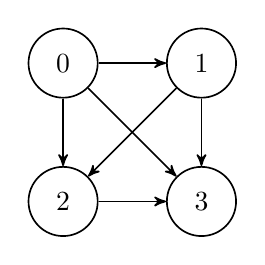
\begin{tikzpicture}[baseline=(current bounding box.center),->,>=stealth', 
	node distance=5em, semithick]
	\tikzstyle{every state}=[fill=none, draw=black, text=black]

	\node[state] (0) {0};
	\node[state] (1) [right of=0] {1};
	\node[state] (2) [below of=0] {2};
	\node[state] (3) [right of=2] {3};

	\path	(0) edge node {} (1)
			(0) edge node {} (2)
			(0) edge node {} (3)
			(1) edge node {} (2)
			(1) edge node {} (3)
			(2) edge node {} (3);

\end{tikzpicture}
}}
	\caption{3-simplex}
	\label{fig:3simplex}
\end{wrapfigure}
Graph analysis of naturally-occurring networks, including neural networks, 
reveals the consistent repetition throughout of small patterns, known as motifs, 
and suggests that network robustness towards perturbation is in part due to the 
presence of these underlying structures, which do not occur at comparable rates 
in random graphs.\cite{Milo824, netmotifs-robustness} \figref{fig:digraph} is an 
example of a directed simplex, a type of motif in which each node is 
unidirectionally connected to every other node, with one node, termed the 
source, only possessing outgoing connections, and another, termed the sink, only 
receiving incoming connections.  In \figref{fig:3simplex}, node 0 is the source, 
and node 3 is the sink.

Since these simplices and other motifs appear in biological neural networks with 
unusual regularity\cite{Reimann2017}, we may be able to take advantage of these 
local properties in reconstruction.


%\subsection{Graph Locality}
%Although physical adjacency is a nonfactor for graphs, we can 

\section{Artificial Neural Networks}
Artificial neural networks, as the name implies, are computational networks, 
usually intended for processing data, inspired by the structure of biological 
networks. They are typically composed of one or more layers, where a layer is a 
set of units that take inputs, either from a previous layer or input data 
directly, and provide output based thereupon. 

\subsection{Feedforward Network Operation}
\begin{wrapfigure}[8]{l}{.35\textwidth}
	\centering
	\vspace{-12pt}
	{\scalebox{.9}{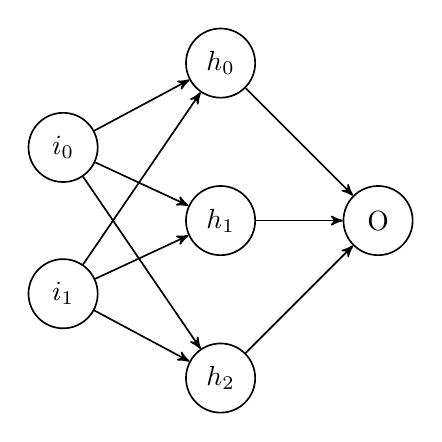
\begin{tikzpicture}[baseline=(current bounding box.center),->,>=stealth', node 
	distance=2cm, semithick]
	\tikzstyle{every state}=[fill=none, draw=black, text=black]
	\node (s) {};
	\node[state] (0) [above=1em of s] {$i_0$};
	\node[state] (1) [below=1em of s] {$i_1$};
	
	\node[state] (3) [right of=s] {$h_1$};
	\node[state] (2) [above of=3] {$h_0$};
	\node[state] (4) [below of=3] {$h_2$};
	
	\node[state] (5) [right of=3] {O};

	\path 	(0) edge node {} (2)
			(0) edge node {} (3)
			(0) edge node {} (4)
			(1) edge node {} (2)
			(1) edge node {} (3)
			(1) edge node {} (4)
			(2) edge node {} (5)
			(3) edge node {} (5)
			(4) edge node {} (5);
\end{tikzpicture}
}}
	\caption{Simple ANN}
	\label{fig:ANN}
\end{wrapfigure}
We will concern ourselves primarily with feedforward networks: those in which 
values move exclusively forward through the layers.
Consider the network in \figref{fig:ANN}. It takes two input values, $i_0$ and 
$i_1$, which constitute its input layer. These inputs are mapped to units 
$h_{0-2}$, which together make up the intermediary layer of this network, often 
referred to as a `hidden' layer.  This transition of values is handled by a 
weight, $w_{ij}$, associated with each connection $i_i \rightarrow h_j$. We can 
consider all of these weights together as a matrix, and the entire transition as 
such:
\begin{equation}
	\begin{bmatrix} h_0 \\ h_1 \\ h_2 \end{bmatrix} = \begin{bmatrix}
w_{00} & w_{01}\\ w_{10} & w_{11}\\ w_{20} & w_{21} \end{bmatrix} \times 
\begin{bmatrix} i_0 \\ i_1 \end{bmatrix}
\end{equation}
Some activation function $f$ is generally applied to the resultant values before 
storing them or calculating the next layer, and in that case we can describe the 
entire transition as $\forall j \in (0,2); h_j = f(w_{j0}i_0 + w_{j1}i_1)$.  
There are a variety of viable activation functions depending on the type of data 
being processed, and they are an important part of how effective ANNs are. For 
example, a network with only two layers but a nonlinear activation function can 
be trained as an arbitrary function approximator.\cite{2006mathematics}
\subsubsection{Training}
The process of optimizing the values in the layer transition matrices is known 
as training, and is often performed by gradient descent via 
backpropagation\cite{Rumelhart}. See \ref{sec:lossandop} for more information on 
this.

\subsection{Convolutional Neural Networks}
\label{subsec:convnets}
Convolutional neural networks provide a method for analyzing data comprising 
many similar features. CNNs as we know them today were popularized by
LeCun et al. in 1998, in a seminal paper\cite{lecun1998gradient} demonstrating 
the use of CNNs for text recognition in images. They recognized the problem 
inherent in using an artificial network scaled to the size of the input (one in 
which the number of input layer units is comparable to the pixels, for instance)
as such:
\begin{quote}
	\ldots\ the main deficiency of unstructured nets for image or speech 
	applications is that they have no built-in invariance with respect to 
	translations, or local distortions of the inputs \ldots\ learning such a 
	task would probably result in multiple units with similar weight patterns 
	positioned at various locations in the input so as to detect distinctive 
	features wherever they appear in the input.\cite[p.~5]{lecun1998gradient}
\end{quote}
This, in a nutshell, describes the utility of convolutional neural networks: for 
data containing multiple features of the same type, such as characters in a 
sentence, training a model that simultaneously considers all parts of the input 
is unecessary; instead, train a \textit{local receptive field}, or filter, 
capable of recognizing that type of feature, and step it across the input.

The benefits of this approach are enormous. Consider text processing: an ANN 
trained, for example, to digitize books by processing an entire page at a time 
would require, at the least, a first layer of similar dimensions to the size of 
a page in pixels. By contrast, a filter just large enough to process a character 
contains many times fewer values, and hence a much lower memory and processing 
load; also recall that having fewer values to optimize renders the training 
process faster and more effective.


\section{Graph Adjacency}
We established in \ref{subsec:motifs} that biological neural networks contain 
high levels of local structure, and in \ref{subsec:convnets} that a 
convolutional architecture, consisting of filters that evaluate small chunks of 
data for particular features, is ideally suited to analyzing such data.

Before making the jump to applying a convolutional architecture to our problem, 
though, we must confront one of the reasons that convolutional filters are 
effective: adjacency. In the case of image analysis, the fact that one pixel or 
group of pixels is next to another is itself important data, as it implies a 
relationship of some nature between those elements. In our problem, there is no 
such data available; local structure in a graph is analagous to adjacency in an 
image, but it is specifically that structure data that we are trying to derive.  
In the second layer of our model, defined in \ref{subsubsec:locality}, we offer 
one solution to this dilemna.

Fortunately, we can apply at least one aspect of a convolutional architecture in 
each layer: while some transforms are defined in terms of the size of the input 
data, all calculations are performed via transposition of a filter across the 
input dataset.


\section{General Operations \& Notation}
Before diving into the specifics of data production, model architecture, and 
training, it's important to establish a firm understanding of the operations 
that will be involved in Chapter \ref{model}.

\subsection{Matrix Operations}
\label{subsec:matops}
Most of the layers in our architecture can be understood with a basic working 
knowledge of matrix math, but some operations may be unfamiliar; we will also 
clarify some notation choices.

\paragraph{Concatenation}
We will periodically need to concatenate matrices on the vertical axis, that is, 
stack them on top of each other; this is the vertical equivalent of matrix 
augmentation. We denote this operation with a horizontal bar between the 
matrices or vectors in question. Example:
\begin{align*}
	\mathbb{A} &= \begin{bmatrix}
		1 & 2 & 3\\
		4 & 5 & 6
	\end{bmatrix} &
	\mathbb{B} &= \begin{bmatrix}
		7 & 8 & 9
	\end{bmatrix} &
	\frac{\mathbb{A}}{\mathbb{B}} = \begin{bmatrix}
		1 & 2 & 3\\
		4 & 5 & 6\\
		7 & 8 & 9
	\end{bmatrix}
\end{align*}
Note that the second dimension of both matrices must be the same; the first, as 
in this example, need not. However, every concatenation in our model involves 
matrices of equal dimensions.

\paragraph{Entrywise Product}
Also known as the Hadamard or Schur product, we denote the entrywise product as 
such:
\begin{equation}
	\underset{x \times y}{\mathbb{C}} = \underset{x \times y}{\mathbb{A}} \odot 
	\underset{x \times y}{\mathbb{B}} \Rightarrow \{c_{ij}\} = \{a_{ij} \times 
	b_{ij}\}
\end{equation}

\subsection{Adjacency Matrices}
\label{subsec:adjacency}
The representation of neural network connectivity that we will focus on is the 
adjacency matrix. For \textit{n} neurons, an adjacency matrix $\mathbb{M}$ will 
be of dimensions $(n \times n)$. A simplistic method of predicting network 
activity at the next discrete timestep, and one that we will use to produce our 
data, is to multiply this matrix by an \textit{n}-vector representing current 
activity at each neuron.  Such an operation appears as follows for $n=3$:
\begin{align}
	\mathbb{S}_{t+1} &= \mathbb{M}\times\mathbb{S}_t =
	\begin{bmatrix}
		a & b & c\\
		d & e & f\\
		g & h & i
	\end{bmatrix}
	\times
	\begin{bmatrix}
		x\\
		y\\
		z
	\end{bmatrix}
	=
	\begin{bmatrix}
		ax + by + cz\\
		dx + ey + fz\\
		gx + hy + iz
	\end{bmatrix}
\end{align}
Thus the activity for a given neuron is defined entirely in terms of network 
activity at the previous timestep and the weights in the adjacency matrix in the 
row corresponding to that neuron. We thereby arrive at a simple expression of 
the mechanics of adjacency matrices: 

\begin{enumerate}
	\item Weights in some row \textit{i} define inputs to neuron \textit{i}
	\item Weights in some column \textit{j} define outputs from neuron 
		\textit{j}
	\item The weight at $\mathbb{M}_{ij}$ defines the connection from neuron 
		\textit{j} to neuron \textit{i}.  \end{enumerate}

Keeping this inverse relationship in mind will help prevent confusion in later 
chapters.

\subsection{Matrix Visualization}
For most data produced by our trained model, be it an output or a weight matrix, 
we will use the following method of visualization as demonstrated in 
\figref{fig:matvisex}. Color depth is  obtained via $C_{ij} = 255 \times 
\frac{\mathbb{M}_{ij}}{max(\mathbb{M})}$.
\begin{figure}[h]
	\centering
	\begin{subfigure}{\textwidth}
		\centering
		\begin{equation*}
			\begin{bmatrix}
				\input{../resources/matEx}
			\end{bmatrix}
		\end{equation*}
		%\caption{Numeric version}
	\end{subfigure}\\
	\vspace{1em}
	\rotatebox{-90}{\scalebox{2}{$\Rightarrow$}}\\
	\vspace{1em}
	\begin{subfigure}{\textwidth}
		\centering
		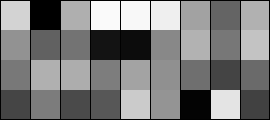
\includegraphics[width=.5\textwidth]{matEx.png}
		\caption{max: 3.97}
	\end{subfigure}
	\caption{The same matrix, in numerical and visual forms}
	\label{fig:matvisex}
\end{figure}\noindent



%! TEX root = /home/hsartoris/sproj/writeup/main.tex
\graphicspath{ {resources/} }
\chapter{Model}
\label{model}
The model trained and tested here represents ... stuff

\section{Data}
\label{sec:data}
Insofar as we treat ANNs as providing arbitrary function approximation, training
a network requires input data representing the known data about the system we
wish to model, as well as output data we wish the network to produce from the
inputs. More generally, input data usually entails information that is easy to 
acquire about the process being modeled, while output data, or labels, 
correspond to a dataset that is difficult to acquire generally. Of course, this 
means that the first step in training a neural network is to assemble a 
sufficiently large set of inputs and outputs in order to fully, or at least 
approximately, characterize the problem at hand.

In our case, we wish to map from (relatively) easily available data about 
biological networks, individual neuron spike times, to network structure. While 
such data exist, generating our own allows us to better analyze the results of 
the algorithm.


\subsection{Generation}
\label{subsec:generation}
In order to demonstrate the validity of our algorithm for graph convolution, we 
opt for a simplified form of the kind of data that would be used in a real-world 
setting.  To this end, we create adjacency matrices representing simple, 
small-\textit{n} toy networks.

\begin{table}[h]
	\centering
	
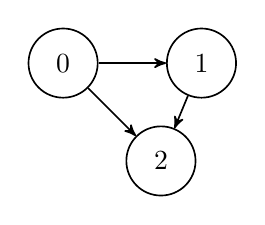
\begin{tikzpicture}[baseline=(current bounding box.center),->,>=stealth', 
	node distance=5em, semithick]
	\tikzstyle{every state}=[fill=none, draw=black, text=black]

	\node[state] (0) {0};
	\node[state] (1) [right of=0] {1};
	\node[state] (2) [below right of=0] {2};

	\path 	(0) edge node {} (1)
			(0) edge node {} (2)
			(1) edge node {} (2);
\end{tikzpicture}

	\hspace{2em}
	\adjacencyT{0 & 0 & 0}{1 & 0 & 0}{1 & 1 & 0}
	\captionof{figure}{Example of 3-neuron network and adjacency matrix.}
	\label{fig:toyex}
\end{table}\noindent
Binary values are used throughout these toy networks: either a connection exists 
or it doesn't; either a `neuron' is spiking or it isn't. To produce spiking 
data, we create an \textit{n}-vector $\mathbb{S}$ representing the current state 
of the toy network, with random neurons already spiking based on a chosen spike 
rate. From here, the process is as in \ref{subsec:adjacency}, where $\mathbb{M}$ 
is the adjacency matrix:
\[
	\underset{n \times n}{\mathbb{M}} \times \underset{n \times 1}{\mathbb{S}^t} 
	= \underset{n \times 1}{\mathbb{S}^{t+1}}
\]
Additonally, $\mathbb{S}^{t+1}$ may have one or more neurons spike randomly, as 
determined by the spike rate of the simulation.\footnote{SEE APPENDIX} All 
values are clipped to the range $[0,1]$, to avoid double spiking. At each step, 
$\mathbb{S}$ is appended to an output matrix, which is saved after simulation is 
complete. For $t$ simulation steps, the completed output has shape $(n \times 
t)$.

Generally, we ran simulations as described for 50 steps\footnote{See 
\ref{subsec:restructuring}}, then saved the resulting output matrix. As many as 
fifty thousand simulations were run for each generator network.
As well as saving the simulated spike trains, we save the adjacency matrix 
describing the generator, in order to provide a target for the model to train 
on.

\subsubsection{Example Data Generation}
Consider the network defined in \figref{fig:toyex}. Supposing that we randomly 
spike neuron 0 at the first step, our initial state appears as such, where 
$\mathbb{O}$ is the output matrix and $\mathbb{R}^0$ is an \textit{n}-vector 
wherein each element has been randomly assigned 0 or 1, based on the spike rate 
of the simulation:
\[
	\mathbb{M} = \begin{bmatrix}
		0 & 0 & 0 \\
		1 & 0 & 0 \\
		1 & 1 & 0
	\end{bmatrix} \qquad
	\mathbb{S}^0 = \begin{bmatrix} 1 \\ 0 \\ 0 \end{bmatrix} \qquad
	\mathbb{O} = \begin{bmatrix} 1 \\ 0 \\ 0 \end{bmatrix} \qquad
	\mathbb{R}^0 = \begin{bmatrix} 0 \\ 1 \\ 0 \end{bmatrix}
\]
We now compute $\mathbb{S}^1$ as above:
\[
	\mathbb{S}^1 = (\mathbb{M} \times \mathbb{S}^0) + \mathbb{R}^0 = 
		\left(\begin{bmatrix}
		0 & 0 & 0 \\
		1 & 0 & 0 \\
		1 & 1 & 0
	\end{bmatrix} \times \begin{bmatrix} 1 \\ 0 \\ 0 \end{bmatrix}\right)
	+ \begin{bmatrix} 0 \\ 1 \\ 0 \end{bmatrix}
	= \begin{bmatrix} 0 \\ 2 \\ 1 \end{bmatrix}
\]
In this case, neuron 1 was spiked randomly, but was also spiked by virtue of its 
connection from 0. Since in this simple model we only consider neurons to be 
either spiking or not, binary values, we clip the values in $\mathbb{S}^1$ to a 
maximum of 1, in order to prevent cases such as this one from causing spikes of 
greater magnitude to propagate through the network. This also prevents neurons 
from double spiking due to multiple inputs being active in the same timestep. 
Thus we have our final value for $\mathbb{S}^1$, and append it to $\mathbb{O}$.
\[
	\mathbb{S}^1 = \begin{bmatrix} 0 \\ 1 \\ 1 \end{bmatrix} \qquad
	\mathbb{O} = \begin{bmatrix}
		1 & 0\\
		0 & 1\\
		0 & 1 \end{bmatrix}
\]
If we were to repeat this process several more times, we might end up with an 
output matrix such as in \figref{fig:exoutput}.
\begin{figure}[H]
\[
	\mathbb{O} = \left[ \mathbb{S}^0 \mid
		\mathbb{S}^1 \mid \mathbb{S}^2 \mid \mathbb{S}^3 \mid \mathbb{S}^4 
	\right] = \begin{bmatrix}
		1 & 0 & 1 & 0 & 0\\
		0 & 1 & 0 & 1 & 0\\
		0 & 1 & 1 & 1 & 1
	\end{bmatrix}
\]
\caption{Example output matrix for a 3-neuron network simulated for five steps.}
\label{fig:exoutput}
\end{figure}\noindent
We can clearly see the effects of neuron 2 having inputs from both other 
neurons. Practically, the number of iterations was usually set to 50.


\subsection{Restructuring}
\label{subsec:restructuring}

\subsubsection{Input Data}
The model accepts data in the form of a spike-time raster plot of dimensions $(n 
\times t)$, where \textit{n} is the number of neurons and \textit{t} is the 
number of timesteps being considered. The axes are reversed in comparison to the 
data created by the generator, and thus in the process of loading in the spike 
trains we transpose the matrices to the expected dimensionality. Additionally, 
it is not always necessary to use the full number of steps generated, depending 
on the size of the generator network in question, as well as its spike rate. In 
such a scenario, we truncate the time dimension appropriately.

For a network accepting \textit{t} timesteps of data from \textit{n} neurons, 
the data fed into the network takes the following form:
\[ \begin{bmatrix}
		x_{11} & x_{12} & \dots & x_{1n}\\
		x_{21} & x_{22} & \dots & x_{2n}\\
		\vdots & \vdots & \ddots & \vdots\\
		x_{t1} & x_{t2} & \dots & x_{tn}
	\end{bmatrix} \]
Applying this process to the data in \figref{fig:exoutput}, including truncating 
the time dimension to four, produces the data in \figref{fig:data+vis}.
\begin{figure}[H]
	\centering
	\begin{subfigure}{.48\textwidth}
		\[
			\begin{bmatrix}
				1 & 0 & 0\\
				0 & 1 & 1\\
				1 & 0 & 1\\
				0 & 1 & 1
			\end{bmatrix}
		\]
		\caption{Transposed output matrix}
	\end{subfigure}
	\begin{subfigure}{.48\textwidth}
		\centering
		
\includegraphics[width=.35\textwidth]{3outex}
		\caption{Graphical representation}
		\label{subfig:3outexgraph}
	\end{subfigure}
	\caption{Transposed and truncated matrix and associated visualization.}
	\label{fig:data+vis}
\end{figure}\noindent
The representation of the matrix in \ref{subfig:3outexgraph} is an example of 
the method we will use to depict matrices containing real values.

\subsubsection{Target Data}
\label{subsubsec:targetdata}
As described in \ref{subsec:generation}, we save the adjacency matrix 
corresponding to the generator along with the simulated spiking files. When an 
adjacency matrix is loaded into the target dataset for training a model, we 
flatten it, from $(n \times n)$ to $(1 \times n^2)$. This allows us to directly 
compare our targets to the outputs of the model, which will be of the same 
dimensionality.

\subsection{Generalizability}
\label{subsec:hotswap}
In most ANN implementations, feeding various data with the same label attached 
to it results in the network learning to ignore the input data and always return 
the desired label, rendering it useless. However, due to the unique structure of 
our model, this sort of overfitting is impossible.\footnote{See 
\ref{subsec:nindependence}} Therefore, we must merely construct a suitably 
representative generator network, meaning that it contains all of the 
inter-neuron relationships we expect to see in the data we ultimately feed in to 
test.

\section{Architecture}
We will first describe the architecture in terms that, while accurate on the 
macro level, do not fully reflect the actual transformations occuring in the 
implemented model. We will then proceed to a mathematically representative 
version, leaving explanation of the batched version of the model to 
\ref{asec:batched}. Additionally, we describe a benchmark model not involving 
locality calculations, in order to provide a point of reference for the efficacy 
of our implementation.

\subsection{Structure \& Computation Details}
\subsubsection{Dimensionality-defining Variables}
Only two values characterize the matrices and transitions involved in the model.  
They are as follows:
\begin{description}
	\item \textit{b}: The number of steps of input data the model considers in a 
		given segment of data.
	\item \textit{d}: The length of the vectors characterizing each potential 
		connection \textit{ij}. This restricts the maximum information about 
		each potential neuron pair that the model can maintain across layer 
		transitions.
\end{description}
We determined effective values for these parameters through experimentation.

While we use the number of nodes in the generator graph, \textit{n}, to 
calculate summations and averages, the structure of our calculations is such 
that no aspects of the model are defined in terms of \textit{n}.

\subsubsection{Omitted Details}
An elementwise activation function\footnote{SEE NN PRINCIPLES} is applied to the 
matrix outputs from each layer. While this is crucial to network function, our 
primary focus in this section is the underlying principles and mathematical 
expressions thereof, and activation is somewhat trivial in comparison. For 
details on the activation functions used, see \ref{sec:activation}.

\subsection{Conceptual Model}
\label{subsec:conceptualmodel}
The operations we describe here represent a per-edge approach to our 
architecture; i.e., the layer transitions are defined in terms of calculations 
applied to single pairs of nodes, as opposed to the whole-matrix operations that 
the architecture as implemented relies on.

\subsubsection{First Transition}
To generate the first layer of the network, we inspect every pair of neurons in 
the input data. Since no pair of neurons is distinguishable from another, the 
comparison applied is the same in all cases: we apply the same convolutional 
filter to all pairs. We achieve this by concatenating the spike train of each 
neuron \textit{i} individually with every other neuron \textit{j}, then 
multiplying by a matrix $\mathbb{W}$ of dimensionality $(d \times 2b)$. To this 
product we add a bias vector, $\mathbb{B}$, of dimensionality $(d \times 1)$.

$\mathbb{W}$ is trained on, and thus the comparison of each pair of spike trains 
is left up to the network. The transition appears as follows, where $\underset{b 
\times 1}{\mathbb{I}_x}$ is the input column at \textit{x}:
\[
	\mathlarger\forall i,j \mid 0 \leq i,j < n: \underset{d \times 
	1}{d_{ij}^\prime} = \underset{d \times 2b}{\mathbb{W}} \times 
	\left(\frac{\mathbb{I}_i}{\mathbb{I}_j}\right) + \underset{d \times 
	1}{\mathbb{B}}
\]
This leaves us with $n^2$ \textit{d}-vectors, each characterizing one potential 
edge \textit{ij}.

\subsubsection{Locality Layer}
\label{subsubsec:locality}
In this layer, we incorporate information from all nodes potentially adjacent to 
each edge \textit{ij}. From our previous layer, we have a matrix of shape $(d 
\times n^2)$ that we will refer to as $\mathbb{D}^{\prime}$, but it will be 
useful to keep in mind an alternate representation of that matrix, one in three 
dimensions, which we shall refer to as $\mathbb{D}_N^{\prime}$. This 
transformation is demonstrated in \figref{fig:transform}.

\begin{figure}[H]
	\centering
	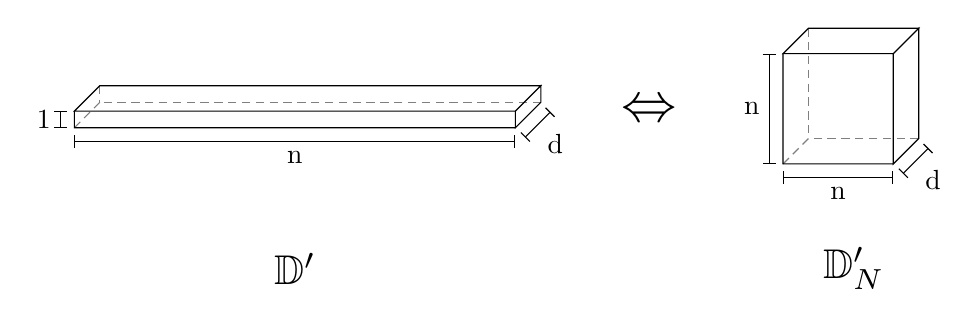
\begin{tikzpicture}
	    \pgfmathsetmacro{\n}{20}
	    \pgfmathsetmacro{\t}{40}
	    \pgfmathsetmacro{\d}{12}
	    \pgfmathsetmacro{\scale}{.07}
		\pic at (2,-1) {annotated cuboid={width=\n*4, height=3, depth=\d, xlabel=n, 
		ylabel=1, zlabel=d, scale=\scale}};
	    \node at (3.7,-1) {\scalebox{2}{$\Leftrightarrow$}};
		\pic at (6.8,-.27) {annotated cuboid={width=\n, height=\n, depth=\d, 
	xlabel=n, ylabel=n, zlabel=d, scale=\scale}};
		\node at (-.8, -3)  {\scalebox{1.5}{$\mathbb{D}^{\prime}$}};
		\node at (6.3, -3) {\scalebox{1.5}{$\mathbb{D}_N^{\prime}$}};
	\end{tikzpicture}
	\caption{Relationship between $\mathbb{D}^{\prime}$ and 
		$\mathbb{D}^{\prime}_N$.}
	\label{fig:transform}
\end{figure}\noindent
Consider some $d_{ij}^{\prime}$ in $\mathbb{D}^{\prime}_N$. Then we can say the 
following:
\begin{enumerate}
	\item $d_{ij}^{\prime}$ represents the connection from \textit{j} to 
		\textit{i} as it may or may not exist in this network, in the form of 
		\textit{d} values of indeterminate meaning
	\item $\mathlarger\forall k \mid 0 \leq k < n$, $d_{jk}^{\prime}$ represents 
		a potential input to \textit{j}
	\item $\mathlarger\forall k \mid 0 \leq k < n$, $d_{ki}^{\prime}$ represents 
		a potential output from \textit{i}
\end{enumerate}
In our determination of the presence or absence of a connection from \textit{j} 
to \textit{i}, we wish to incorporate information from these potentially 
connected nodes; i.e., these inputs and outputs represent potential neighbors in 
terms of graph locality. To achieve this, we perform the following 
computations\footnote{Actually, it's much more elegant.} for each $\underset{d 
\times 1}{d_{ij}}$:
\begin{minipage}{\textwidth}
\begin{subequations}
	\centering
	\begin{align}
		\label{eq:ID}
		\underset{d \times 1}{\mathbb{I}} &= \frac{1}{n} \sum_{k=0}^{n-1} 
		d_{jk}^{\prime} & \underset{d \times 1}{\mathbb{O}} &= \frac{1}{n} 
		\sum_{k=0}^{n-1} d_{ki}^{\prime}\\
		\label{eq:IDOD}
		\underset{d \times 1}{\mathbb{I_D}} &= \underset{d \times 
			d}{\mathbb{W}_{in}^\prime} \times \left(\mathbb{I} \odot 
		d_{ij}^{\prime}\right) & \underset{d \times 1}{\mathbb{O_D}} &= 
		\underset{d \times d}{\mathbb{W}_{out}^\prime} \times \left(\mathbb{O} 
		\odot d_{ij}^{\prime}\right)
	\end{align}
	\text{Here we arrive at the output, $d_{ij}^{\prime\prime}$:}
	\begin{equation}
		\underset{d \times 1}{d_{ij}^{\prime\prime}} = \underset{d \times 
		2d}{\mathbb{W}_{tot}^\prime} \times 
		\left(\frac{\mathbb{I_D}}{\mathbb{O_D}}\right) + \underset{d \times 
		1}{\mathbb{B}^\prime}
		\label{eq:dijO} 
	\end{equation}
\end{subequations}
Conceptually, in \eqref{eq:ID} we first average all potential inputs to and 
outputs from potential edge \textit{ij}. Then, we compute an entrywise product 
($\odot$) of these vectors with the vector describing the edge in question, 
$d_{ij}^{\prime}$. While we have integrated locality data into the results thus 
far, the network has not been allowed any processing over the resultant data, 
which we rectify by multiplying the input and output vectors with separate 
dimensionality-preserving $(d \times d)$ matrices. We thus arrive at 
\eqref{eq:IDOD}, with vectors $\mathbb{I_D}$ and $\mathbb{O_D}$ representing 
edge \textit{ij} with inputs and outputs, respectively, taken into 
consideration. In \eqref{eq:dijO}, we arrive at $d_{ij}^{\prime\prime}$ by 
multiplying a third weight matrix by the vertical concatenation of 
$\mathbb{I_D}$ and $\mathbb{O_D}$.  This matrix, $\mathbb{W}_{tot}^\prime$, 
allows the network to optimize for whichever elements in $\mathbb{I_D}$ and 
$\mathbb{O_D}$ are most important in the prediction of \textit{ij}.  
Additionally, a bias vector, $\mathbb{B}^\prime$, is added to this product, and 
at this point we have $d_{ij}^{\prime\prime}$ as it will be seen by the next 
layer of the network.\footnotemark
%The three matrices involved, $\mathbb{W}_{in}^\prime$, 
%$\mathbb{W}_{out}^\prime$, and $\mathbb{W}_{tot}^\prime$, are trained on by the 
%optimizer\footnote{SEE OPTIMIZER SECION IN TRAINING}, allowing the model to 
%learn optimal processing and combinations to facilitate predictions.
\end{minipage}
\footnotetext{Disregarding the activation function}

Our concatenation approach in \eqref{eq:dijO} stands in contrast to the strategy 
taken in \eqref{eq:IDOD}, where integration of the input and output data is 
forced via entrywise product computation. For discussion of this attribute, see 
\ref{subsec:localops}.

Note again that none of the computations involved in this layer are dependent on 
\textit{n}; as the summations are averaged, the values contained in their 
resultant vectors will be of similar magnitude for any number of neurons under 
consideration. After executing this algorithm for each $d_{ij}^{\prime}$, we are 
left with another $(d \times n^2)$ output matrix, $\mathbb{D}^{\prime\prime}$.

\subsubsection{Final Transition}
The shift from $(d \times n^2)$ is comparatively simple, being only a 
dimensionality reduction:
\begin{equation}
	\label{eq:conceptfinal}
	\mathlarger\forall d_{ij}^{\prime\prime} \in \mathbb{D}^{\prime\prime}:
	\underset{1 \times 1}{d_{ij}^f} = \underset{1 \times d}{\mathbb{W}^f} \times 
	\underset{d \times 1}{d_{ij}^{\prime\prime}}
\end{equation}
This leaves us with a $(1 \times n^2)$ matrix, which, following application of 
an activation function as defined in \ref{subsec:finalactivation} and 
transposition to $(n \times n)$, we treat as the adjacency matrix of the 
generator associated with the input data.

\subsection{Matrix Model}
\label{subsec:matmodel}
While the processes defined in \ref{subsec:conceptualmodel} are accurate 
representations of the operations undertaken in our model, they are generally 
defined in terms of individual vectors, with iteration over all vectors 
necessarily implied. This does not take advantage of the computational abilities 
of modern GPU computing, and, if implemented as such, would render training 
times astronomical. Therefore, we create a version of our model executed 
entirely in terms of matrix operations, ideal for GPU execution.

\subsubsection{First Layer}
\label{subsubsec:matfirstlayer}
In the first layer, we wish to compare each input vector against every input 
vector by way of concatenation and matrix multiplication to reduce 
dimensionality. To achieve this via matrix operations is fairly simple. We first 
define two helper matrices:
\begin{align*}
	\underset{n \times n^2}{\mathbb{E}} &= \begin{bmatrix}
			\underset{1 \times n}{\mathbbm{1}} & \dots & 0\\
			\vdots & \ddots & \vdots \\
		0 & \dots & \underset{1 \times n}{\mathbbm{1}} \end{bmatrix}\\
		\underset{n \times n^2}{\mathbb{T}} &= \begin{bmatrix}
	I_n & \mid & \dots & \mid I_n \end{bmatrix}
\end{align*}
With $\underset{b \times n}{\mathbb{I}}$ as our input data, the first layer 
transition is as follows:
\begin{equation}
	\label{eq:matfirst}
	\underset{d \times n^2}{\mathbb{D}^\prime} = \underset{d \times 
	2b}{\mathbb{W}}
	\left(\frac{\mathbb{I}\times\mathbb{E}}{\mathbb{I}\times\mathbb{T}}\right) + 
	\left(\underset{d \times 1}{\mathbb{B}}\times\underset{1 \times 
	n^2}{\mathbbm{1}}\right)
\end{equation}
\paragraph{Example:}
Consider a model for which $b=3$ and $n=2$. Suppose that we have the following 
input matrix: \[ \mathbb{I} = \begin{bmatrix} 1 & 1\\ 1 & 0\\ 0 & 1\end{bmatrix}
\]
Then our helper matrices would appear as such:
\[
	\mathbb{E} = \begin{bmatrix}
		1 & 1 & 0 & 0\\
		0 & 0 & 1 & 1
	\end{bmatrix}
	\hspace{2em}
	\mathbb{T} = \begin{bmatrix}
		1 & 0 & 1 & 0\\
	0 & 1 & 0 & 1 \end{bmatrix}
\]
And our matrix stack:
\[
	\mathbb{I} = \begin{bmatrix} 1 & 1\\ 1 & 0\\ 0 & 1\end{bmatrix}
	\hspace{3em}
	\frac{\mathbb{I} \times \mathbb{E}}{\mathbb{I} \times \mathbb{T}} = 
	\begin{bmatrix}
		1 & 1 & 1 & 1\\
		1 & 1 & 0 & 0\\
		0 & 0 & 1 & 1\\
		1 & 1 & 1 & 1\\
		1 & 0 & 1 & 0\\
		0 & 1 & 0 & 1
	\end{bmatrix}
\]
Thus, over all of the columns in the resulting stack, every vector in 
$\mathbb{I}$ is paired with all such vectors, including itself.

\subsubsection{Locality Layer}
\label{subsubsec:matconvlayer}
In the conceptual model, there are two averages of sums involved in processing 
each vector in $\mathbb{D}^\prime$; one over the horizontal axis of 
$\mathbb{D}^\prime_N$, and the other over the vertical axis. These can be found 
in \eqref{eq:ID}. Consider two vectors $d_{ij}, d_{il} \in \mathbb{D}^\prime_N$.  
For both of these vectors, the average input vector is the same, its calculation 
being only dependent on the first coordinate, $i$. The inverse holds for vectors 
with the same second coordinate. Thus we see that these calculations need only 
be performed once for each $k \in [0,n)$. Considering the $(d \times n^2)$ 
representation of the current data matrix $\mathbb{D}^\prime$, the `vertical' 
summation of column \textit{i} appears as such:
\[
	\mathbb{O} = \sum_k d^\prime_{ki} = \mathbb{D}^\prime_{0+i} + 
	\mathbb{D}^\prime_n + \mathbb{D}^\prime_{2n + i} + \dots + 
	\mathbb{D}^\prime_{(n-1)n + i}
\]
This is the inverse of the tile operation executed by $\mathbb{T}$ in the first 
layer, and that same matrix allows us to compute all outputs to all edges 
simultaneously:
\begin{equation}
	\underset{d \times n}{\mathbb{O}} = \frac{1}{n} \left(\mathbb{D}^\prime 
	\times \mathbb{T}^\top\right)
\end{equation}
Similarly, to calculate the sum of row j in $\mathbb{D}^\prime_N$:
\[
	\mathbb{I} = \sum_k d^\prime_{jk} = \sum_{l=j}^{j + n-1} \mathbb{D}^\prime_l
\]
This is the inverse of the expand operation executed by $\mathbb{E}$, and once 
again we can use that same matrix to compute all edge inputs simultaneously:
\begin{equation}
	\underset{d \times n}{\mathbb{I}} = \frac{1}{n}\left(\mathbb{D}^\prime 
	\times \mathbb{E}^\top \right)
\end{equation}
These operations allow us to avoid ever transposing $\mathbb{D}^\prime$, instead 
allowing us to work directly on it.

For both $\mathbb{I}$ and $\mathbb{O}$, we still need to pair the vectors within 
with the appropriate vector in $\mathbb{D}^\prime$. To accomplish this, we must 
expand both matrices to $(d \times n^2)$. 

For some vector $\mathbb{I}_x$, we wish to pair it with all vectors $d_{kx} \in 
\mathbb{D}^\prime_N \mid k \in [0,n)$. In terms of $\mathbb{D}^\prime$, these 
vectors map to $\mathbb{D}^\prime_{kn+x}$; i.e., we wish to create a matrix into 
which we distribute a given vector in $\mathbb{I}$ \textit{n} times, \textit{n} 
columns apart. Once again, we already have a matrix specifically capable of this 
operation: $\mathbb{T}$.  Similarly, we wish to pair any given vector 
$\mathbb{O}_x$ with all vectors ${d_{xk} \in \mathbb{D}^\prime_N \mid k \in 
[0,n)}$, which correspond with $\mathbb{D}^\prime_{xn + k}$: for each vector in 
$\mathbb{O}$, we broadcast it into a $(d \times n^2)$ matrix such that it 
repeats \textit{n} times. Yet again, an established matrix will complete this 
task: $\mathbb{E}$. Thus our intermediary steps for this layer are quite similar 
to \eqref{eq:IDOD}:
\begin{subequations}
	\label{eq:matsecond}
	\begin{align}
		\underset{d \times n^2}{\mathbb{I_D}} &= \underset{d \times 
		d}{\mathbb{W}_{in}^\prime} \times \left(\left(\mathbb{I} \times 
	\mathbb{T}\right) \odot \mathbb{D}^\prime\right) & \underset{d \times 
n^2}{\mathbb{O_D}} &= \underset{d \times d}{\mathbb{W}_{out}^\prime} \times 
\left(\left(\mathbb{O} \times \mathbb{E}\right) \odot \mathbb{D}^\prime\right)
	\end{align}
	\text{And we arrive at the matrix expression of the locality layer:}
	\begin{equation}
		\label{eq:matsecondfinal}
		\underset{d \times n^2}{\mathbb{D}^{\prime\prime}} = \underset{d \times 
			2d}{\mathbb{W}_{tot}^\prime} \times 
			\left(\frac{\mathbb{I_D}}{\mathbb{O_D}}\right) + \left(\underset{d 
			\times 1}{\mathbb{B}^\prime} \times \underset{1 \times 
	n^2}{\mathbbm{1}}\right)
	\end{equation}
\end{subequations}

\subsubsection{Final Layer}
\label{subsubsec:matfinallayer}
The operation for the matrix version of the final layer is effectively the same 
as \eqref{eq:conceptfinal}:
\begin{equation}
	\label{eq:matfinal}
	\underset{1 \times n^2}{\mathbb{D}^f} = \underset{1 \times d}{\mathbb{W}^f} 
	\times \underset{d \times n^2}{\mathbb{D}^{\prime\prime}}
\end{equation}

\subsection{Benchmark Model}
\label{subsec:benchmark}
The model we provide as a benchmark mimics our model in its first 
\eqref{eq:matfirst} and final \eqref{eq:matfinal} layers. The difference lies in 
the second layer: where in \eqref{eq:matsecond} we perform a variety of 
transforms to incorporate locality data, here this layer is entirely defined by 
the following equation:
\begin{equation}
	\label{eq:benchsecond}
	\underset{d \times n^2}{\mathbb{D}^{\prime\prime}} = \underset{d \times 
	d}{\mathbb{W}^\prime} \times \underset{d \times n^2}{\mathbb{D}^\prime} + 
	\underset{d \times 1}{\mathbb{B}^\prime} \times \underset{1 \times 
	n^2}{\mathbbm{1}}
\end{equation}

\subsection{\textit{n}-independence}
\label{subsec:nindependence}
\subsubsection{Trainable Values}
Between all of the operations defined in \ref{subsec:matmodel} (and equivalently 
in \ref{subsec:conceptualmodel}), the following matrices are the only values 
over which the optimizer can perform gradient descent:
\subparagraph{First Layer}
\begin{itemize}
	\item[$\ubb{W}{d}{2b}$:] weight matrix used to merge columns of input data
	\item[$\ubb{B}{d}{1}$:] bias vector added to every $\mathbb{D}^\prime_k \mid 
		k \in [0,n)$.
\end{itemize}

\subparagraph{Locality Layer}
\begin{itemize}
	\item[$\underset{d \times d}{\mathbb{W}_{in}^\prime}$:] weight matrix used 
		to process data entering an edge
	\item[$\underset{d \times d}{\mathbb{W}_{out}^\prime}$:] weight matrix used 
		to process data exiting an edge
	\item[$\underset{d \times 2d}{\mathbb{W}_{tot}^\prime}$:] weight matrix used 
		to merge the data produced by $\underset{d \times 
			d}{\mathbb{W}_{out}^\prime}$ and $\underset{d \times
			d}{\mathbb{W}_{in}^\prime}$
	\item[$\underset{d \times 1}{\mathbb{B}^\prime}$:] bias vector added to 
		every $\mathbb{D}^{\prime\prime}_k \mid k \in [0,n)$.
\end{itemize}

\subparagraph{Final Layer}
\begin{itemize}
	\item[$\underset{1 \times d}{\mathbb{W}}^f$:] weight matrix used to collapse 
		all $n^2$ vectors into $n^2$ scalars.
\end{itemize}

\subparagraph{Benchmark Model}
Our benchmark model shares first and final layer structures with the overall 
model, leading to its having the same optimizable parameters for those layers.  
Its second layer retains the bias vector $\mathbb{B}^\prime$, but that and a 
single $(d \times d)$ matrix $\mathbb{W}^\prime$ are the only optimizable 
values.


\subsubsection{Implications}
As noted previously, none of these matrices are dependent on \textit{n}.  
Furthermore, even in the matrix model (\ref{subsec:matmodel}), the weight 
matrices operate individually on each \textit{ij} vector, and the same bias is 
added to each vector.  Because the network is not provided any trainable 
\textit{n}-scale values, all calculation and training is done per node pair.  
This obviates the typical neural network problem of overfitting to its training 
dataset to the point it simply memorizes appropriate outputs.\footnote{See 
\ref{sec:overfitting}} Additionally, this allows for application of a trained 
model to data produced by generators of a different size than those used to 
train the model. Because our model operates entirely on local graph features, 
the only requirement for such an application is that the training data contain a 
set of features also representative of the new data.


\chapter{Training}

\section{Datasets}


\section{Matrix Initialization}

\section{Hyperparameter Optimization}

\subsection{Loss Optimization}

\subsubsection{Loss Function}

\subsubsection{Optimizer Function}


%! TEX root = /home/hsartoris/sproj/writeup/main.tex
\graphicspath{ {resources/models/} } 

\chapter{Results}
\label{results}
\section{Overfitting}
\label{sec:overfitting}
\setlength{\columnsep}{20pt}
\begin{wraptable}[8]{r}{.4\textwidth}
	\captionsetup{justification=centering}
	\vspace{-20pt}
	\begin{tabular}{lr}
		\textit{b} (timesteps) & 8\\
		\textit{d}& 5\\
		Batch size& 32\\
		Training steps& 20000\\
		Learning rate& .0005\\
		Training samples& 18000\\
		Validation samples& 4500
	\end{tabular}
	\vspace{-5pt}
	\captionof{figure}{\linespread{1.2}\selectfont{}Training parameters for null 
		hypothesis networks}
	\label{fig:nullparams}
\end{wraptable}
As discussed in \ref{subsec:hotswap} and \ref{subsec:nindependence}, the unique 
structure of our model prevents it from overfitting to a particular generator 
topology, allowing us to create a single generator containing connections 
representative of the types of data we expect to analyze with the trained model.
We demonstrate this aspect of our architecture in two test cases: by training 
models on an empty dataset paired with one adjacency matrix throughout, and 
training with a random dataset paired with that same adjacency matrix.

\subsection{Empty Data}
\label{subsec:empty}
We ran a combined 100 training sessions of the benchmark model and our 
convolutional model, with parameters as defined in \figref{fig:nullparams}, on a 
dataset whose inputs contained only zeroes and whose target was the adjacency 
matrix in \figref{fig:2simplex+adjacency}. For both models, exactly two losses 
and corresponding outputs repeatedly occurred (\figref{fig:empty_loss}), with 
the models demonstrating a total inability to memorize the target data.

\begin{figure}[h]
	\centering
	\begin{subfigure}{.45\textwidth}
		\centering
		\begin{tabular}{cccc}
				   &  0 &  1 &  2\\\cline{2-4}
			\mc{0} & .3 & .3 & .3\\
			\mc{1} & .3 & .3 & .3\\
			\mc{2} & .3 & .3 & .3
		\end{tabular}
		\caption{loss: $0.\overline{6}$}
		\label{subfig:empty_loss0}
	\end{subfigure}
	\begin{subfigure}{.45\textwidth}
		\centering
		\begin{tabular}{llll}
			  & 0 & 1 & 2\\\cline{2-4}
			\mc{0} & 0 & 0 & 0\\
			\mc{1} & 0 & 0 & 0\\
			\mc{2} & 0 & 0 & 0
		\end{tabular}
		\caption{loss: 1.0}
		\label{subfig:empty_loss1}
	\end{subfigure}
	\caption{Predictions and losses when training on an empty dataset}
	\label{fig:empty_loss}
\end{figure}

\subsection{Random Data}
\label{subsec:random}
\begin{wrapfigure}[7]{r}{.25\textwidth}
	\vspace{-20pt}
	\adjacencyT{0 & .5 & .5}{.5 & 0 & .5}{.5 & .5 & 0}
	\caption{Average prediction for random data. loss: 0.5}
	\label{fig:random_output}
\end{wrapfigure}
For this trial, all model parameters were identical to those in 
\ref{subsec:empty}. In this case, however, the data fed into the network 
consisted of raster plots whose items had been randomly assigned to 0 or 1.  
While the results were somewhat less consistent, over the course of 100 training 
sessions, the models that were able to converge to a minimum loss predicted the 
matrix in \figref{fig:random_output} the overwhelming majority of the time. 

\subsection{Analysis}
While the results of \ref{subsec:random} are at first confusing, given the per 
edge architecture of our model, this result is not particularly surprising: in 
the first layer transition, every spike vector is compared against every other 
spike vector, including itself. Thus the model was in fact able identify a set 
of connections \textit{ij} exhibitng a particular feature: in the first layer, 
$\mathbb{I}_i = \mathbb{I}_j$. Because it could reliably identify these pairs, 
meaning the optimizer could target them, gradient descent minimized loss 
appropriately and adjusted the weight matrices such that, for such an 
\textit{ij} pair, $\mathbb{D}^{\prime\prime}_{ij} = 0$.

For the remainder of the potential connections, the model, lacking any way to 
distinguish between them, found an equilibrium value that, when applied to the 
remaining connections, minimized loss. Note that both uniformly increasing or 
decreasing the nonzero weights in \figref{fig:random_output} increases loss.

The same is true of the results in \ref{subsec:empty}, with the output in 
\figref{subfig:empty_loss1} particularly illustrative of the problem of entropy 
traps in neural networks. For models that converged to this output, the initial 
seeding of the weight and bias matrices was such that the fastest decreases in 
loss were found by adjusting trainable values to produce an empty matrix. Once 
there, uniformly increasing the output values would initially increase the loss, 
preventing the network from pushing upward and eventually reaching the lower 
loss state of \figref{subfig:empty_loss0}.



\section{3-neuron generator}
\label{results_3neur}
We now consider a generator network consisting of three nodes connected as in 
\figref{fig:2simplex+adjacency}. All weights are binary, and a spike rate of .25 
was used.\footnote{SEE APPENDIX	for information on spike rates} 

\begin{table}[h]
	\centering
	\captionsetup{margin=5em}
	
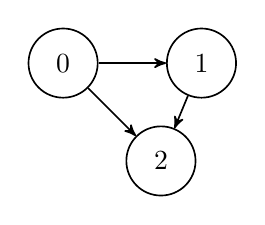
\begin{tikzpicture}[baseline=(current bounding box.center),->,>=stealth', 
	node distance=5em, semithick]
	\tikzstyle{every state}=[fill=none, draw=black, text=black]

	\node[state] (0) {0};
	\node[state] (1) [right of=0] {1};
	\node[state] (2) [below right of=0] {2};

	\path 	(0) edge node {} (1)
			(0) edge node {} (2)
			(1) edge node {} (2);
\end{tikzpicture}

	\hspace{2em}
	\begin{tabular}{llll}
		& 0 & 1 & 2\\\cline{2-4}
		\mc{0} & 0 & 0 & 0\\
		\mc{1} & 1 & 0 & 0\\
		\mc{2} & 1 & 1 & 0
	\end{tabular}
	\captionof{figure}{Network structure and adjacency matrix of the generator.  
	(Reproduced from Figure \ref{fig:toyex})}
	\label{fig:2simplex+adjacency}
\end{table}\noindent
Reconstructing this simplified graph allows us to demonstrate that our 
convolutional approach is capable of reconstruction.  Furthermore, the small 
generator size requires few timesteps and a small interlayer featurespace; i.e., 
$b,d<10$.  This results in a relatively simple set of transitions, allowing us 
to explore and understand the inner workings of the network.

\subsection{Example Model}
\label{subsec:3neurex}
In order to demonstrate the internal mechanics of our model, we trained on data 
produced by the generator given in \figref{fig:2simplex+adjacency}, with 
parameters as given in \ref{fig:3neur_loss+params}. In this example, small 
values of \textit{b} and \textit{d} were used in order to allow for better 
comprehension and visualization of the internal mechanics; the practical effect 
of this is that relatively small matrices were available for the model to 
optimize, making each value adjustment more impactful on output, and thus each 
training step more dramatic.  These are acceptable limitations, however, insofar 
as they provide a more comprehensible model struture.

\begin{table}[ht]
	\centering
	\begin{minipage}{.48\textwidth}
	\resizebox{\textwidth}{!}{
		\begin{tikzpicture}
			\begin{semilogyaxis} [xlabel=Step, ylabel=Loss, scaled x 
				ticks=false,
				axis lines*=left,
				xtick={1,3750,7500,11250,15000},
				extra y ticks={.05,.5}, extra y tick style={grid=major},
%				ytick={0,.1,.5,1}, 
				yticklabel style={	/pgf/number format/precision=2,
									/pgf/number format/fixed}]
				\addplot [color=black] table [x=Step, y=Loss, col sep=comma, 
			mark=none, smooth] {../resources/models/3neurEx/losses};
			\end{semilogyaxis}
		\end{tikzpicture}
	}
	\end{minipage}
	\hfill
	\begin{minipage}{.48\textwidth}
		\centering
		\begin{tabular}{lr}
			b (timesteps) & 8\\
			d& 5\\
			Batch size& 32\\
			Learning rate& .0005\\
			Training samples& 17984\\
			Validation samples& 4512
		\end{tabular}
	\end{minipage}
	\captionof{figure}{Training loss and parameters for model described in 
	\ref{subsec:3neurex}. The loss here is somewhat choppier than usual, due to 
the limited matrix size made available to the model.}
	\label{fig:3neur_loss+params}
\end{table}


\subsection{Trained Network Operation}
Here, we will consider a single item of data as it travels through the model 
trained in \ref{subsec:3neurex}.

\label{subsec:trainedoperation}
\begin{figure}[h]
	\centering
	\begin{subfigure}{.15\textwidth}
		\centering
		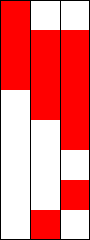
\includegraphics[width=.75\textwidth]{3neurEx/fullRun/0_py/input.png}
		\caption{Input\\(max: 1.0)}
		\label{subfig:3neur_in}
	\end{subfigure}
	\hspace{.5em}
	\begin{subfigure}{.35\textwidth}
		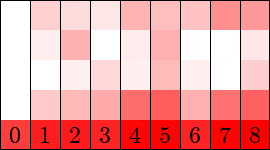
\includegraphics[width=\textwidth]{3neurEx/fullRun/0_py_num/layer0/4out.png}
		\caption{Output of first layer\\(max: 4.33)}
	\end{subfigure}
	\hspace{1em}
	\begin{subfigure}{.35\textwidth}
		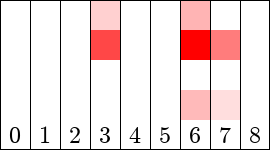
\includegraphics[width=\textwidth]{3neurEx/fullRun/0_py_num/layer1/7out.png}
		\caption{Output of second layer\\(max: 3.2)}
		\label{subfig:3neur_out1}
	\end{subfigure}
	\\
	\begin{subfigure}{.35\textwidth}
		\centering
		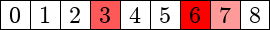
\includegraphics[width=\textwidth]{3neurEx/fullRun/0_py_num/layerf/0out.png}
		\caption{Output of final layer\\(max: 30.97)}
		\label{subfig:3neur_outf}
	\end{subfigure}
	\begin{subfigure}{.3\textwidth}
		\centering
		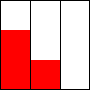
\includegraphics[width=.5\textwidth]{3neurEx/fullRun/0_py/pred.png}
		\caption{Prediction\\(max: 1.0)}
		\label{subfig:3neur_pred}
	\end{subfigure}
	\caption{Path of data through network. Transparency for each value is scaled 
	relative to the maximum value found in the matrix.}
	\label{fig:3neur_run}
\end{figure}\noindent
In \figref{fig:3neur_run}, we demonstrate the progression of 
\ref{subfig:3neur_in} through the trained model. The final layer, including 
activation\footnote{See \ref{subsec:finalactivation}}, produces an $n^2$-vector 
which, when reshaped into an $(n \times n)$ matrix, is an exact match for the 
target, with all connections located and weighted appropriately.\footnote{While 
	$[1,0]$ and $[2,0]$ are predicted to be exactly 1.0, the precise value of 
	$[2,1]$ in the final prediction is 0.999999999957586, which we consider to 
be accurate enough.}
\subsubsection{Brief Analysis}
\paragraph{Final Layer}
\begin{wrapfigure}[5]{r}{.25\textwidth}
	\centering
	\vspace{-15pt}
	
\includegraphics[width=.25\textwidth]{3neurEx/fullRun/0_py/layerf/weights.png}
	\caption{Final weights\\(max: 7.31)}
	\label{fig:3neur_flayer}
\end{wrapfigure}
The final layer consists only of multiplying its weights 
(\figref{fig:3neur_flayer}) by the output from the locality layer, and it is 
thus relatively easy to intepret what the model has learned at this stage. As 
the first two values of of the weight matrix are strongly positive, we can 
conlude that the first two values in each vector in the output from the previous 
layer are highly important in the determination of connection presence, with 
some weight also placed on the fourth item.

\paragraph{Locality Layer Functionality}

Note that, following the locality layer (\ref{subfig:3neur_out1}), the model has 
located the existent connections: if we transpose \ref{subfig:3neur_out1} from 
$(d \times n^2)$ to $(n \times n \times d)$, as in \figref{fig:transform}, the 
columns with high values, 3, 6, and 7, correspond with \textit{d}-vectors 
$[1,0]$, $[2,0]$, and $[2,1]$, respectively. These tuples each correspond with a 
connection present in the adjacency matrix (\figref{fig:toyex}) the model is 
trying to predict.
\vspace{\baselineskip}

\noindent Proceeding any deeper than this, the operation of the model becomes 
fairly opaque. Nonetheless, we have included the data for this full run in 
\ref{asec:fullrun}.

\section{Higher-order Datasets}
\label{sec:localitybroken}
Because a 3-node generator not does contain much in terms of locality, we 
created a graph structure containing slightly more complex relationships to 
benchmark our model on; that generator can be found in \figref{fig:10neur}.
 
\begin{table}[h]
	\centering
	\vspace{-5pt}
	{\scalebox{.9}{
	{\scalebox{.9}{
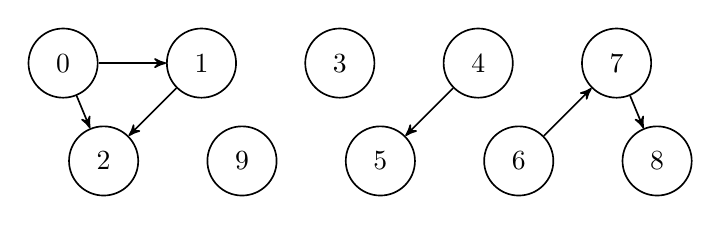
\begin{tikzpicture}[baseline=(current bounding box.center),->,>=stealth', 
	node distance=5em, semithick]
	\tikzstyle{every state}=[fill=none, draw=black, text=black]

	\node[state] (0) {0};
	\node[state] (1) [right of=0] {1};
	\node[state] (2) [below left of=1] {2};
	\node[state] (3) [right of=1] {3};
	\node[state] (4) [right of=3] {4};
	\node[state] (5) [below left of=4] {5};
	\node[state] (6) [right of=5] {6};
	\node[state] (7) [above right of=6] {7};
	\node[state] (8) [right of=6] {8};
	\node[state] (9) [below left of=3] {9};

	\path 	(0) edge node {} (1)
			(0) edge node {} (2)
			(1) edge node {} (2)
			(4) edge node {} (5)
			(6) edge node {} (7)
			(7) edge node {} (8);
\end{tikzpicture}

	
}}
	\hspace{1em}
	\begin{tabular}{ccccccccccc}
			   & 0 & 1 & 2 & 3 & 4 & 5 & 6 & 7 & 8 & 9\\\cline{2-11}
		\mc{0} &   &   &   &   &   &   &   &   &   &  \\
		\mc{1} & \bf1 &   &   &   &   &   &   &   &   &  \\
		\mc{2} & \bf1 & \bf1 &   &   &   &   &   &   &   &  \\
		\mc{3} &   &   &   &   &   &   &   &   &   &  \\
		\mc{4} &   &   &   &   &   &   &   &   &   &  \\
		\mc{5} &   &   &   &   & \bf1 &   &   &   &   &  \\
		\mc{6} &   &   &   &   &   &   &   &   &   &  \\
		\mc{7} &   &   &   &   &   &   & \bf1 &   &   &  \\
		\mc{8} &   &   &   &   &   &   &   & \bf1 &   &  \\
		\mc{9} &   &   &   &   &   &   &   &   &   &  
	\end{tabular}
	}}
	\captionof{figure}{Ten neuron generator and adjacency matrix. For purposes 
	of clarity, all zero values in the matrix have been omitted.}
	\label{fig:10neur}
\end{table}\noindent

We trained 100 model/benchmark pairs on the data produced by this generator; the 
losses and parameters of the best-performing models of each type can be found in 
\figref{fig:9neur_loss+params}. The results, in which the losses of both types 
of networks stayed extremely close, demonstrate that, while the locality-based 
approach is able to reconstruct networks, it does not offer substantive 
improvement over the much more straightforward benchmark model, at least in the 
cases that we have considered.  An example run can be found in 
\figref{fig:samepred}.
\begin{table}[ht]
	\centering
	\begin{minipage}{.48\textwidth}
	\resizebox{\textwidth}{!}{
		\begin{tikzpicture}
			\begin{semilogyaxis} [xlabel=Step, ylabel=Loss, scaled x 
				ticks=false,
				axis lines*=left,
				xtick={1,3750,7500,11250,15000},
				extra y ticks={.05,.5}, extra y tick style={grid=major},
%				ytick={0,.1,.5,1}, 
				yticklabel style={	/pgf/number format/precision=2,
									/pgf/number format/fixed}]
				\addplot [color=black] table [x=Step, y=Loss, col sep=comma, 
			mark=none, smooth] {../resources/models/3neurEx/losses};
			\end{semilogyaxis}
		\end{tikzpicture}
	}
	\end{minipage}
	\hfill
	\begin{minipage}{.48\textwidth}
		\centering
		\begin{tabular}{lr}
			b (timesteps) & 8\\
			d& 5\\
			Batch size& 32\\
			Learning rate& .0005\\
			Training samples& 17984\\
			Validation samples& 4512
		\end{tabular}
	\end{minipage}
	\captionof{figure}{Training loss and parameters for model described in 
	\ref{subsec:3neurex}. The loss here is somewhat choppier than usual, due to 
the limited matrix size made available to the model.}
	\label{fig:3neur_loss+params}
\end{table}

\begin{figure}[h]
	\centering
	\hfill
	\begin{subfigure}{.2\textwidth}
		\centering
		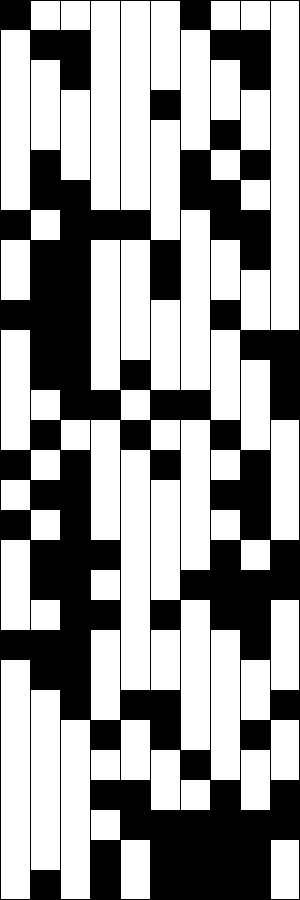
\includegraphics[width=\textwidth]{9neur/conv1/input.png}
		\caption{Input}
	\end{subfigure}
	\hspace{2em}
	\begin{minipage}{.65\textwidth}
		\centering
	\begin{subfigure}{.9\textwidth}
		\centering
		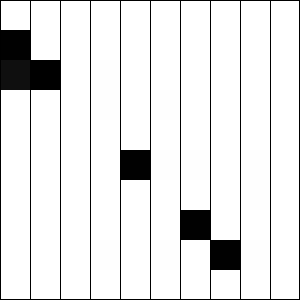
\includegraphics[width=.45\textwidth]{9neur/conv1/pred.png}
		\caption{Locality-based model prediction}
	\end{subfigure}\\
	\begin{subfigure}{.9\textwidth}
		\centering
		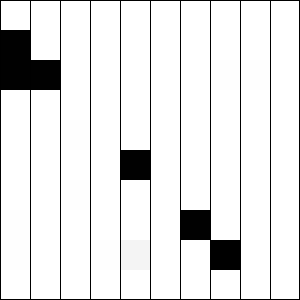
\includegraphics[width=.45\textwidth]{9neur/dumb1/pred.png}
		\caption{Benchmark model prediction}
	\end{subfigure}
	\end{minipage}
	\caption{Example of data from generator defined in \figref{fig:10neur}, 
	passed through the locality-based and benchmarks models.}
	\label{fig:samepred}
\end{figure}\noindent
\newpage
The same results were found with generators of various sizes and topologies, 
although none larger than that in \figref{fig:10neur} were used. It is 
important, however, not to overstate the importance of this comparison, 

\section{Applicability Beyond Training Data}
As described in \ref{subsec:hotswap}, the fact that our model is trained on data 
produced by only one generator is of little consequence; due to its structure, 
the only information it can learn is relational, per neuron pair. Consider the 
following examples, in which data was produced from several generator networks 
and run through the models previously described.

\subsection{Model trained on \ref{results_3neur}}
TODO: add examples of input and output data to 3.2.1 and 3.2.2.

\subsubsection{Inverted Network}
\begin{table}[h]
	\centering
	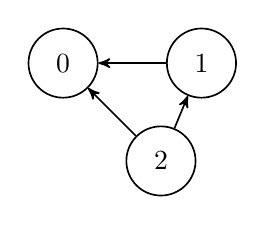
\begin{tikzpicture}[baseline=(current bounding box.center),->,>=stealth', 
	node distance=5em, semithick]
	\tikzstyle{every state}=[fill=none, draw=black, text=black]

		\node[state] (0) {0};
		\node[state] (1) [right of=0] {1};
		\node[state] (2) [below right of=0] {2};
	
		\path 	(2) edge node {} (1)
				(2) edge node {} (0)
				(1) edge node {} (0);
	\end{tikzpicture}
	\hspace{2em}
	\begin{tabular}{l|lll}
		  & 0 & 1 & 2\\
		\hline
		0 & 0 & 1 & 1\\
		1 & 0 & 0 & 1\\
		2 & 0 & 0 & 0
	\end{tabular}
	\captionof{figure}{Inverted version of \figref{fig:2simplex+adjacency}}
	\label{fig:2simplexVar1}
\end{table}
\noindent Despite being a complete inversion of the generator used to train the 
model in \ref{results_3neur}, reconstruction of this network is simple.
\begin{figure}[h]
	\graphicspath{{resources/models/3neurEx/fullRun/invert/}}
	\begin{subfigure}{.16\textwidth}
		\centering
		
\includegraphics[width=\textwidth]{input.png}
		\caption{Input\\(max: 1.0)}
	\end{subfigure}
	\hspace{1em}
	\begin{minipage}{.5\textwidth}
		\centering
		\begin{subfigure}{.8\textwidth}
			\centering
			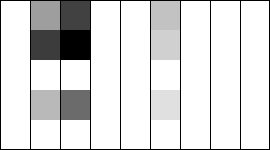
\includegraphics[width=\textwidth]{layer1/7out.png}
			\caption{Output of locality layer\\(max: 5.29)}
		\end{subfigure}\\
		\vfill
		\begin{subfigure}{.8\textwidth}
			\centering
			\igtw{layerf/0out.png}
			\caption{Output of final layer\\(max: 72.06)}
		\end{subfigure}
	\end{minipage}
	\begin{minipage}{.25\textwidth}
		\centering
		\vspace{-10pt}
		\vspace{1em}
		\adjacencyT{0.0 & 1.0 & 1.0}{0.0 & 0.0 & 1.0}{0.0 & 0.0 & 0.0}
		\begin{subfigure}{\textwidth}
			\centering
			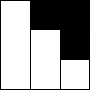
\includegraphics[width=.7\textwidth]{pred.png}
			\caption{Prediction\\(max: 1.0)}
		\end{subfigure}
	\end{minipage}
	\caption{Data from \figref{fig:2simplexVar1}}
\end{figure}
		

%\begin{table}[h]
%	\centering
%	\begin{minipage}{.1\textwidth}
%		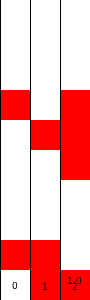
\includegraphics[width=\textwidth]{3neurEx/var1/input.png}
%	\end{minipage}
%	\hspace{2em}
%	{\scalebox{2}{$\Rightarrow$}}
%	\hspace{2em}
%	\begin{tabular}{l|lll}
%		  & 0 & 1 & 2\\
%		\hline
%		0 & .01 & 1.00 & 1.00\\
%		1 & .01 & .02 & 1.00\\
%		2 & 0 & .02 & .01
%	\end{tabular}
%\end{table}

\subsubsection{Cyclical Network}
\label{subsec:cyclical}
\begin{table}[h]
	\centering
	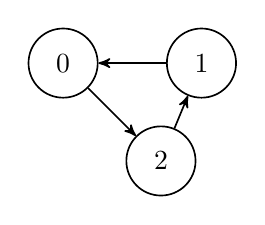
\begin{tikzpicture}[baseline=(current bounding box.center),->,>=stealth', 
	node distance=5em, semithick]
	\tikzstyle{every state}=[fill=none, draw=black, text=black]

		\node[state] (0) {0};
		\node[state] (1) [right of=0] {1};
		\node[state] (2) [below right of=0] {2};
	
		\path 	(2) edge node {} (1)
				(0) edge node {} (2)
				(1) edge node {} (0);
	\end{tikzpicture}
	\hspace{2em}
	\begin{tabular}{l|lll}
		  & 0 & 1 & 2\\
		\hline
		0 & 0 & 1 & 0\\
		1 & 0 & 0 & 1\\
		2 & 1 & 0 & 0
	\end{tabular}
	\captionof{figure}{Cyclical 3-neuron network}
	\label{fig:2simplexVar2}
\end{table}

\noindent For a cyclical network, the situation is not quite so simple. Due to 
the perpetual propagation of spikes through the generator, additional random 
spiking can cause the input data to become an impenetrable mess. Tempering the 
spike rate to 0.05 produces workable data, but the results are neither so clean 
nor
consistent as for terminating networks.  




%! TEX root = /home/hsartoris/sproj/writeup/main.tex
\chapter{Discussion}

\section{Potential Improvements}

\subsection{Algorithm}
Detail issues with summing inputs and outputs, and propose alternative algorithm 
here. Note issues with implementation.

\subsection{Optimizer}
I think it's in the paper about ELU or SELU that they use a ramping up learn 
rate and then decline. That might be ideal for the original, concatenation-based 
implemenation of the network, to avoid pushing it down the gradient too fast and 
zeroing out the convolutional matrix sections.


%! TEX root = /home/hsartoris/sproj/writeup/main.tex
\begin{appendices}
	\chapter{Parameter Optimization Miscellanea}
	\section{Data}
	\subsection{Spike Rate Determination}
	As seen in section \ref{subsec:cyclical}, oversaturated data hamstrings the 
	ability of our model to perform accurate reconstructions. As the 

	\chapter{Model}
	\section{Batched Architecture Calculations}
	\label{asec:batched}
	In order to allow processing of many pieces of data at once, the matrix 
	model defined in \ref{subsec:matmodel} was adapted to a batched format.  
	Given input matrices of shape $(b \times n)$, the actual input to the model 
	is now of shape $(batchSize \times b \times n)$. As previously discussed, 
	iteration across lists or dimensions is not a computationally efficient 
	option. Therefore we use \texttt{tf.einsum}, an implementation of Einstein 
	Sums. This allows, for example, the multiplication of two matrices, one of 
	dimension $(i \times j \times k)$, and the other of dimension $(h \times 
	j)$. An appropriate function call might appear as
	\texttt{tf.einsum(`hj,ijk->ihk', mat2, mat1)}. The result is equivalent to 
	the iterative multiplication of the $(h \times j)$ matrix across all 
	\textit{i}, without the computational overhead of CPU involvement. Every 
	matrix multiplication in our model is implemented using this functionality.


\end{appendices}


\bibliographystyle{abbrv}
\bibliography{total}

\end{document}
